\section{Database Design}

\subsection{Entity-Relationship Diagram}
The system architecture revolves around the central entity \textbf{Investors}. All operational tables connect directly to \textbf{Investors} via the \texttt{InvestorID} foreign key, accurately reflecting the core objective: tracking individual investor behavior over time to detect panic selling[cite: 1]. 

The schema defines the following core relationships:
\begin{itemize}
    \item \textbf{Investors 1-N Trades}: An investor executes multiple trades across different tickers over time.
    \item \textbf{Investors 1-N Portfolios}: The system records a daily asset snapshot for each investor.
    \item \textbf{Investors 1-N BehaviorSignals}: The system calculates and stores behavioral signals for each observation day.
    \item \textbf{Investors 1-N Warnings}: The system automatically generates warnings when an investor's \texttt{PanicScore} exceeds the defined threshold.
    \item \textbf{MarketData} operates independently. It contains no direct foreign key to \textbf{Investors} because it represents aggregated market conditions, not individual investor data.
\end{itemize}

\begin{figure}[h!]
\begin{center}
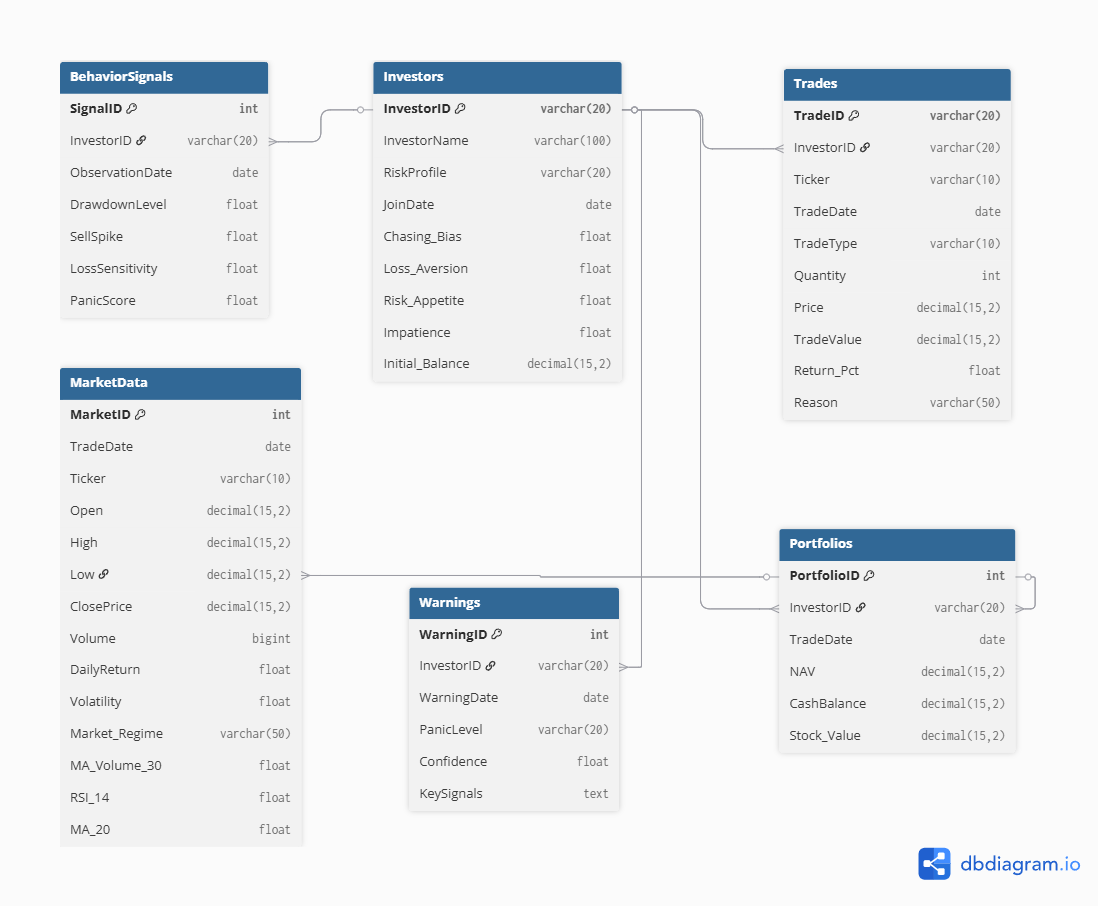
\includegraphics[width=\textwidth]{Images/ERD.png}
\end{center}
\caption{Entity-Relationship Diagram — Panic Selling Detection System}
\end{figure}

\subsection{Relational Schema}
We translate the Entity-Relationship diagram into six relational tables. The design adheres strictly to the single responsibility principle, ensuring each table stores only one specific category of information. This structured data model satisfies the technical soundness criteria for the database architecture[cite: 1].

\begin{itemize}
    \item \textbf{Table 1: Investors}
    \begin{itemize}
        \item Stores demographic information and psychological parameters.
        \item \textbf{PK}: \texttt{InvestorID VARCHAR(20)}
        \item The psychological parameters (\texttt{Chasing\_Bias}, \texttt{Loss\_Aversion}, \texttt{Risk\_Appetite}, \texttt{Impatience}) are system-specific configurations used to control simulation behavior rather than raw empirical data.
        \item \texttt{RiskProfile} categorizes investors into three groups: FOMO, RATIONAL, and NOISE.
    \end{itemize}

    \item \textbf{Table 2: MarketData}
    \begin{itemize}
        \item Stores historical price action for 9 Vietnamese stock tickers.
        \item \textbf{PK}: \texttt{MarketID AUTO\_INCREMENT}
        \item A \texttt{UNIQUE} constraint on \texttt{(TradeDate, Ticker)} prevents data duplication.
        \item \texttt{Market\_Regime} stores the classified market state (derived from \texttt{DailyReturn} and \texttt{Future\_Return}) directly in the table to accelerate simulation read operations.
    \end{itemize}

    \item \textbf{Table 3: Trades}
    \begin{itemize}
        \item Records the complete transaction history.
        \item \textbf{PK}: \texttt{TradeID VARCHAR(20)}
        \item \textbf{FK}: \texttt{InvestorID} $\rightarrow$ \texttt{Investors}
        \item \texttt{Reason} captures behavioral labels (PANIC\_SELL, FOMO\_BUY, RATIONAL\_BUY, DISTRIBUTION\_SELL). This acts as the ground truth label for calculating the \texttt{SellSpike} during feature engineering.
        \item \texttt{Return\_Pct} records the exact profit or loss percentage at the time of sale, driving the \texttt{LossSensitivity} metric.
    \end{itemize}

    \item \textbf{Table 4: Portfolios}
    \begin{itemize}
        \item Captures the end-of-day asset snapshot.
        \item \textbf{PK}: \texttt{PortfolioID AUTO\_INCREMENT}
        \item Records \texttt{NAV} (Net Asset Value), calculated as \texttt{CashBalance + Stock\_Value}.
        \item Utilizes a time-series design (one row per investor per trading day) to support rapid calculation of the \texttt{DrawdownLevel}.
    \end{itemize}

    \item \textbf{Table 5: BehaviorSignals}
    \begin{itemize}
        \item Stores the results of daily feature engineering computations.
        \item \textbf{PK}: \texttt{SignalID AUTO\_INCREMENT}
        \item Designed as a separate entity from \texttt{Trades} and \texttt{Portfolios} because it contains derived data calculated over a rolling 30-day window, not raw transaction logs.
        \item Database triggers monitor the \texttt{PanicScore} in this table to determine warning generation.
    \end{itemize}

    \item \textbf{Table 6: Warnings}
    \begin{itemize}
        \item Stores risk alerts generated automatically by system triggers.
        \item \textbf{PK}: \texttt{WarningID AUTO\_INCREMENT}
        \item \texttt{PanicLevel} categorizes risk into High, Medium, or Low.
        \item \texttt{KeySignals} uses a JSON string format to list the specific technical and behavioral signals triggering the alert.
        \item \texttt{Confidence} reflects the \texttt{PanicScore} value at the exact moment of trigger execution, providing a reliability metric for the warning.
    \end{itemize}
\end{itemize}

\subsection{Synthetic Dataset Design}
Due to strict privacy regulations and the unavailability of granular, individual-level transaction logs from brokerage firms, we engineered a synthetic data generation pipeline. This pipeline simulates realistic trading behaviors and psychological biases observed in the Vietnamese retail stock market.

\subsubsection{Market Data Generation}
We sourced actual historical price data for 9 major Vietnamese tickers (VIC, VHM, HPG, FPT, VCB, SSI, VPB, BCM, MSN) for the year 2025 using the \texttt{vnstock} library. We calculated standard technical indicators, including \texttt{MA\_20}, \texttt{RSI\_14}, \texttt{MA\_Volume\_30}, and \texttt{DailyReturn}. 

To guide the simulation agents, we classified the market into five distinct regimes based on the current \texttt{DailyReturn} and the 5-day \texttt{Future\_Return}:

\begin{table}[h!]
\centering
\begin{tabular}{|l|l|l|}
\hline
\textbf{Regime} & \textbf{Condition} & \textbf{Significance} \\ \hline
EXPLOSION & \texttt{DailyReturn} > 2\% & Abnormally strong upward momentum \\ \hline
PANIC & \texttt{DailyReturn} < -2\% & Severe market drop, panic conditions \\ \hline
SIDEWAY\_ACCUMULATION & \texttt{Future\_Return} > 3\% & Price consolidation prior to an uptrend \\ \hline
SIDEWAY\_DISTRIBUTION & \texttt{Future\_Return} < -3\% & Price distribution prior to a downtrend \\ \hline
SIDEWAY\_NOISE & All other conditions & Normal market fluctuations \\ \hline
\end{tabular}
\caption{Market Regime Classification Logic}
\end{table}

\subsubsection{Investor Profiles}
We simulated a base of 1,000 virtual investors, categorizing them into three behavioral risk profiles:
\begin{itemize}
    \item \textbf{FOMO (30\%):} Configured with high \texttt{Chasing\_Bias} (0.75-0.99), high \texttt{Loss\_Aversion}, and high \texttt{Impatience}. These agents exhibit a strong tendency to buy during EXPLOSION regimes and sell off aggressively during PANIC regimes.
    \item \textbf{RATIONAL (50\%):} Assigned low psychological parameters (0.01-0.35). These agents make execution decisions based purely on technical analysis signals (e.g., RSI, MA crossovers) and resist emotional trading.
    \item \textbf{NOISE (20\%):} Assigned mid-range parameters (0.3-0.7). These agents execute trades at random intervals without clear technical or behavioral patterns.
\end{itemize}
The pipeline assigns each investor a randomized \texttt{Initial\_Balance} ranging from 10 million to 5 billion VND and a \texttt{JoinDate} spanning the last 9 years.

\subsubsection{Transaction Simulation}
Each trading day, an \texttt{InvestorAgent} assesses the \texttt{Market\_Regime} and \texttt{ClosePrice} of the 9 tickers, deciding whether to BUY, SELL, or HOLD. The decision logic dictates that during a PANIC regime, FOMO investors have a high statistical probability of executing a \texttt{PANIC\_SELL} on their entire position. Conversely, during an EXPLOSION regime, they tend to execute \texttt{FOMO\_BUY} orders. RATIONAL investors remain largely inactive unless specific technical criteria are met.

We incorporated price slippage to increase realism: fill prices during a PANIC regime simulate a 1-3\% drop below the \texttt{ClosePrice}, while EXPLOSION fills are 0.5-2\% higher.

\begin{table}[h!]
\centering
\begin{tabular}{|l|r|}
\hline
\textbf{Table Name} & \textbf{Row Count} \\ \hline
Investors & 1,000 \\ \hline
MarketData & 2,160 \\ \hline
Trades & 48,250 \\ \hline
Portfolios & 240,000 \\ \hline
BehaviorSignals & 210,000 \\ \hline
Warnings & 4,125 \\ \hline
\end{tabular}
\caption{Database Record Statistics Following Simulation}
\end{table}

\subsection{Behavioral Feature Engineering}
The system derives three distinct behavioral signals from the raw transaction and portfolio data. We calculate these signals daily for each investor using a rolling 30-day lookback window. These features capture different dimensions of panic selling behavior.

\subsubsection{DrawdownLevel}
This metric quantifies the peak-to-trough decline in portfolio asset value.
$$DrawdownLevel = \min\left(1.0,\ \max\left(0,\ \frac{NAV_{peak} - NAV_{final}}{NAV_{peak}}\right) \times 5\right)$$
\textit{Explanation:} The formula measures the asset drop from its 30-day peak. We apply a $5\times$ multiplier to amplify the signal, as a 20\% portfolio drawdown in real-world retail trading typically indicates severe distress and triggers panic behaviors.

\subsubsection{SellSpike}
This metric measures the concentration of fear-driven sell orders.
$$SellSpike = \frac{\text{SELL orders labeled PANIC or DISTRIBUTION}}{\text{Total SELL orders in 30 days}}$$
\textit{Explanation:} A high \texttt{SellSpike} value indicates that the investor is liquidating positions abruptly without a predefined strategy, reacting heavily to short-term market regimes.

\subsubsection{LossSensitivity}
This metric evaluates the investor's willingness to accept realized losses.
$$LossSensitivity = \frac{\text{SELL orders with Return\_Pct} < 0}{\text{Total SELL orders in 30 days}}$$
\textit{Explanation:} Panic-stricken investors frequently close positions at a loss to exit the market entirely, prioritizing immediate cash over potential recovery.

\subsubsection{PanicScore and Thresholds}
The system aggregates the three signals into a final score:
$$PanicScore = 0.4 \times DrawdownLevel + 0.4 \times SellSpike + 0.2 \times LossSensitivity$$
\textit{Weighting Logic:} \texttt{DrawdownLevel} and \texttt{SellSpike} carry higher weights (0.4) because they are direct, immediate manifestations of panic. \texttt{LossSensitivity} receives a lower weight (0.2) because selling at a loss can occasionally represent a disciplined, pre-planned stop-loss execution by a RATIONAL investor.

The trigger evaluates the \texttt{PanicScore} to categorize risk levels:
\begin{itemize}
    \item \textbf{High:} $PanicScore \ge 0.6$
    \item \textbf{Medium:} $PanicScore \ge 0.4$
    \item \textbf{Low:} $PanicScore < 0.4$
\end{itemize}

\begin{figure}[ht]
\begin{center}
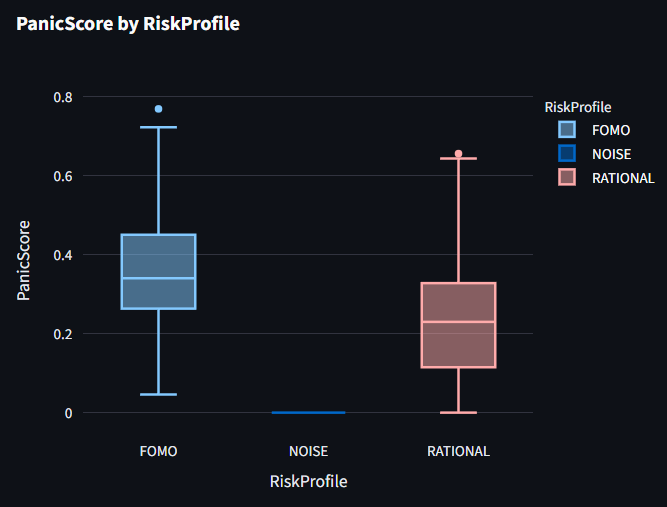
\includegraphics[width=0.8\textwidth]{Images/boxplot.png}
\end{center}
\caption{PanicScore distribution by RiskProfile}
\end{figure}

As illustrated in Figure 2, the FOMO cohort exhibits the highest median \texttt{PanicScore} ($\sim0.35$) with a wide interquartile range, validating their highly volatile and reactive trading behavior. The NOISE group maintains a \texttt{PanicScore} near 0, as their random executions rarely cluster into identifiable panic patterns. The RATIONAL group shows a wider distribution than NOISE due to higher overall trading volume, but their disciplined execution prevents them from reaching the high-risk panic thresholds.